\section{Key Game Features}

\begin{figure}[H]
  \centering
  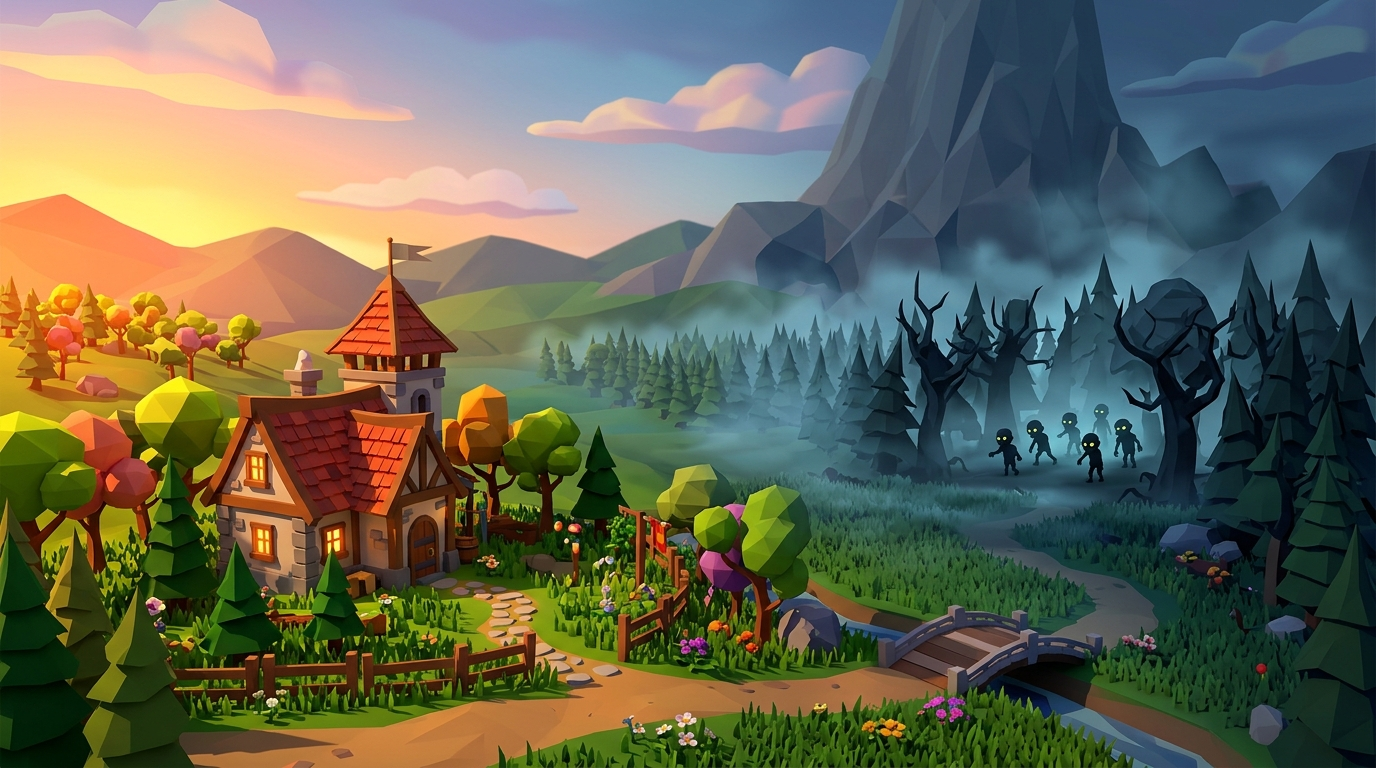
\includegraphics[width=\textwidth]{images/main-menu-visual.jpg}
  \caption{Project visual used for the main-menu presentation: a protected house facing an approaching zombie threat.}
  \label{fig:main-menu-visual}
\end{figure}

\textit{Zombie House 3D} is designed around readable, complementary systems rather than a large number of unrelated mechanics. Figure~\ref{fig:main-menu-visual} communicates the intended contrast between the player's safe base and the hostile enemy area; the following features turn that setting into a playable defense round.

\subsection{Player-driven combat and planting}
\begin{itemize}
  \item \textbf{Third-person movement and melee:} the player can move around the map, adjust the camera, and fight enemies that reach the defensive line.
  \item \textbf{Plant-based defense:} plantable squares and plant data allow the player to place defenders deliberately instead of depending only on direct attacks.
  \item \textbf{Resource decisions:} the sun economy connects resource collection and plant costs, requiring the player to decide when and where to invest in defense.
  \item \textbf{Flexible interaction:} selected plants can be placed or removed, which supports correction and adaptation during a round.
\end{itemize}

\subsection{Enemy waves, progression, and feedback}
\begin{itemize}
  \item \textbf{Wave defense:} zombies follow routes toward the house, attack when they arrive, and are cleared through coordinated player and plant damage.
  \item \textbf{Multiple enemy forms:} the integration setup includes standard zombie behavior and a spider/zombie variant, making the enemy system extensible.
  \item \textbf{Clear game states:} house health, wave progression, and win/lose panels communicate whether the player is holding the defense or has completed the round.
  \item \textbf{Presentation support:} day, cloudy, and night map variants, a minimap, menu navigation, background music, and action SFX reinforce orientation and feedback.
\end{itemize}

\begin{figure}[H]
  \centering
  \begin{tikzpicture}[
    node distance=0.55cm and 0.7cm,
    feature/.style={draw=blue!55!black, rounded corners=3pt, fill=blue!6, minimum width=3.3cm, minimum height=1.2cm, align=center, font=\small},
    flow/.style={-{Stealth[length=2mm]}, thick, blue!55!black}
  ]
    \node[feature] (player) {Player movement\\and melee};
    \node[feature, right=of player] (plants) {Sun economy\\and plant defense};
    \node[feature, below=of player] (waves) {Zombie routes\\and wave pressure};
    \node[feature, below=of plants] (feedback) {House health, UI,\\minimap, and audio};
    \draw[flow] (player) -- (plants);
    \draw[flow] (plants) -- (feedback);
    \draw[flow] (waves) -- (player);
    \draw[flow] (waves) -- (feedback);
  \end{tikzpicture}
  \caption{The main gameplay features form one defense loop: enemy pressure drives player and plant actions, while the house and UI provide the round's feedback.}
  \label{fig:feature-loop}
\end{figure}
